\section{Kvalitativ risikovurdering}

	{\bf Problem 2) Forestill deg at du er medlem i et prosjektteam som har blitt gitt i oppgave 
	å utvikle et nytt produkt for byggeindustrien. Ved bruk av en kvalitativ matrise for 
	risikoanalyse skal det gjøres en risikovurdering for et prosjekt basert på følgende 
	informasjon: }

	\begin{table}[H]
		\begin{tabular}{ p{9cm} p{3cm} }
			\hline
			Identifiserte risikofaktorer & Sannsynlighet \\ \hline
			1. Sentrale prosjektmedlemmer trekkes fra prosjektet & 1. Høy \\
			2. Endring av økonomiske nedgangstider & 2. Lav \\
			3. Kutt av prosjektmidler & 3. Medium \\
			4. Endring i prosjektomfang (scope) & 4. Høy \\
			5. Dårlig ytelse av spesifikasjon & 5. Lav \\
			\hline

		\end{tabular}
	\end{table}

	{\bf Basert på denne informasjonen, hvordan kan du rangere konsekvensene for hvert av de
	identifiserte risikofaktorene? Hvorfor? Konstruer risikomatrisen og klassifiser hver 
	av risikofaktorene i matrisen.}


	\subsection{Konsekvenser}

		\begin{enumerate}
			\item{\bf Sentrale prosjektmedlemmer trekkes fra prosjektet:} 
			Når sentrale medlemmer trekkes fra et prosjekt betyr det store konsekvenser for flere ledd.
			For det første må det brukes tid og ressurser på å erstatte prosjektmedlemmet, eller at
			de resterende prosjektmedlemmene må ta over arbeidsoppgavene om kompetansen i prosjektgruppa
			kan dekke alle oppgaver. Ved at en person forsvinner fra et prosjekt mister man ikke bare
			kompetanse, men også prosjekterfatinger som er blitt gjort underveis. En ny person som kommer
			inn bruker ofte ekstra tid på å komme seg inn i et prosjekt ved å måtte komme inn i rutiner
			og sette seg inn ved prosjektets ståsted. Siden dette påvirker flere ledd i et prosjekt 
			blir dette satt med en høy konsekvens. 
			{\bf \color{red} Høy konsekvens}
			\item{\bf Økonomiske nedgangstider:} i byggeindustrien er økonomisk status veldig viktig,
			med tanke på kjøp fra leverandører og salg til kunder. Ved økonomsik nedgang kan det ofte bli
			vanskelig å få solgt. Feks ved nybygg er det vanlig å starte et prosjekt og selge underveis
			for å dekke utgifter. Ved økonomisk nedgang kan man stå i en posisjon der kunder ikke er
			kjøpesterke nok til å ville kjøpe noe ved tanke på økonomisk risiko. 
			Uten å ha økonomien på plass kan slike byggeprosjketer stoppe opp. Dette vil igjen 
			påvirke leverandører i den betydningen at det ikke er nok penger til å betale for det
			man har avtalt å kjøpe eller har kjøpt. Andre konsekvenser er prosjektstopp og store 
			forsinkelser som igjen fører til stort ressurs- og økonomisk tap. 
			Økonomiske nedgangstider er en noe som er vanskelig å gjøre noe med, noe som gjør
			at konsekvensen blir veldig høy. {\bf \color{red} Høy konsekvens}
			\item {\bf Kutt av prosjektmidler:} i byggebransjen er man avhengig av prosjektmidler 
			fordi man opererer med forskjellige leverandører. Ved kutt av prosjektmidler kan man 
			risikere at billigere materialer blir kjøpt, noe som kan føre til dårlig kvalitet eller
			uforutsette risikoer relater til kvalitetskutt. Siden slike kutt kan koordineres og kan 
			holdes under kontroll ved god prosjektstyring vil dette settes som en middels konsekvens. 
			{\bf \color{orange} Middels konsekvens}
			\item {\bf Endring i prosjektomfang (scope):} i byggebransjen vil endring i prosjektomfang
			bli tatt imot forskjellig etter hvor i prosjektsyklusen man er. Hvis det er i en tidlig
			fase vil det bli tatt imot godt fordi selve byggingen ikke er i gang. Om man i en sen fase
			oppdager feil og ender scope vil det mest sannsynlig fås store økonomiske konsekvenser. 
			Det er ikke bra å finne ut at materiale man har brukt i bunn ikke holder konstruksjonen
			når man er halvveis i byggingen (ja, muligens banalt, men det har skjedd).
			Siden det ikke er spesifisert hvor i syklusen det er setter jeg det til middels konsekvens. 
			{\bf \color{orange} Middels konsekvens}
			\item {\bf Dårlig ytelse av spesifikasjon:}
			{\bf \color{orange} Middels konsekvens}
		\end{enumerate}

	\clearpage
	\subsection{Risiko = Sannsynlighet x Konsekvens}

		\begin{tabular}{ p{8cm} l l l}
			\hline
			Identifiserte risikofaktorer & Sann. & Kons. & Risiko \\ \hline
			1. Sentrale prosjektmedlemmer trekkes fra prosjektet & Høy & Høy & Høy\\
			2. Endring av økonomiske nedgangstider & Lav & Høy & Middels \\
			3. Kutt av prosjektmidler & Middels & Middels & Middels \\
			4. Endring i prosjektomfang (scope) & Høy & Middels & Høy \\
			5. Dårlig ytelse av spesifikasjon & Lav & Middels & Lav \\
			\hline
		\end{tabular}

		\begin{figure}[H]
			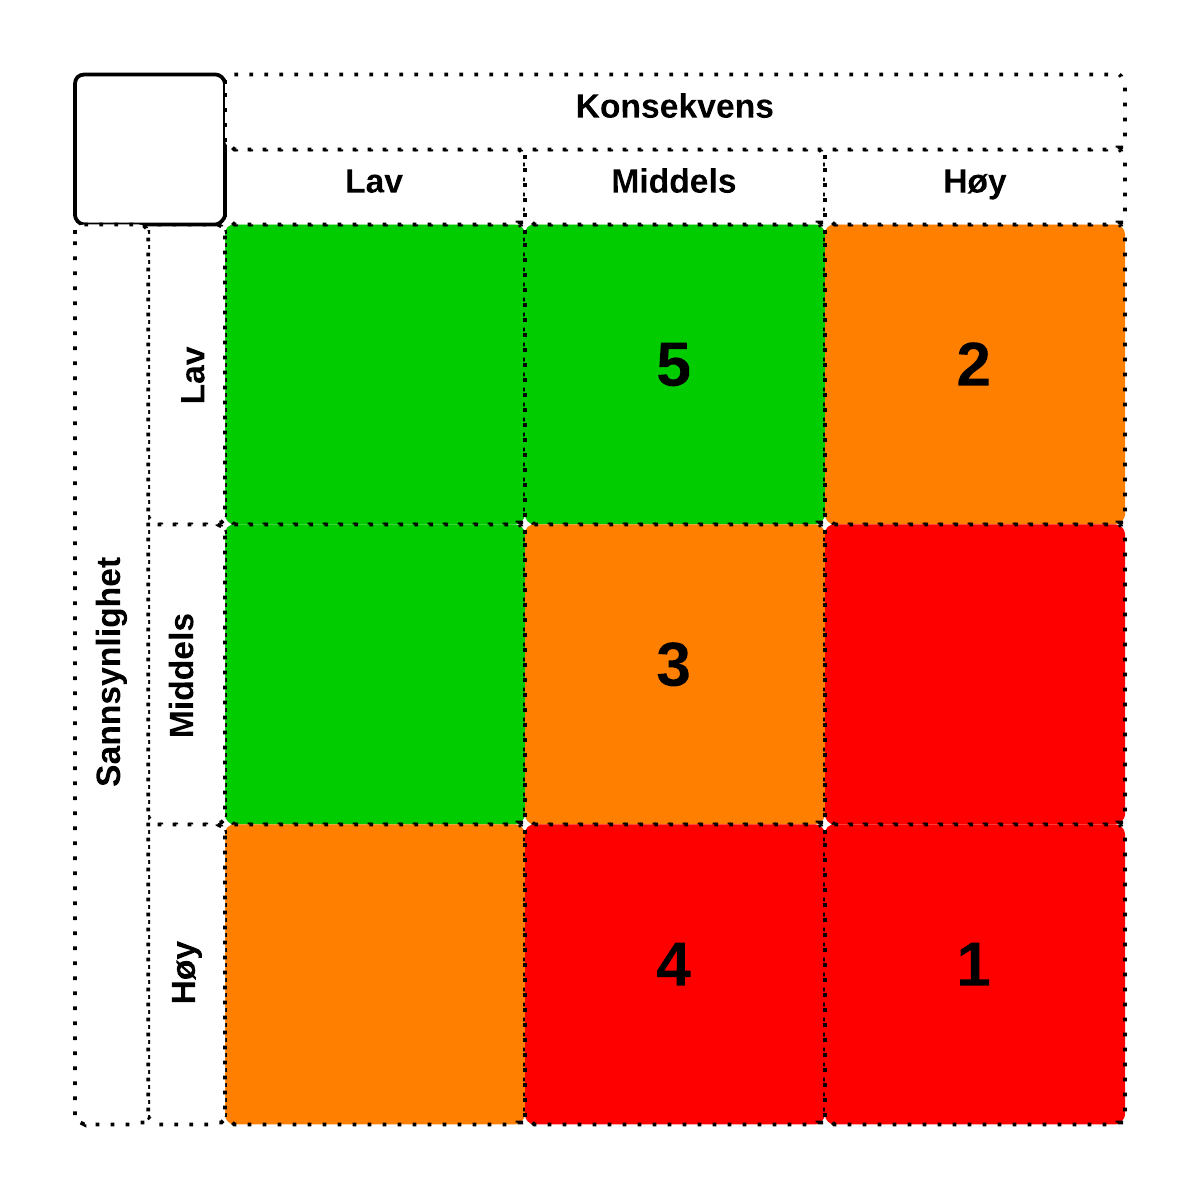
\includegraphics[width=\textwidth]{riskMatrix.png}
			\caption{Risikomatrise}
		\end{figure}

